\chapter{指令系统}
\section{寻址方式}
\subsection{立即寻址}
操作数包含在指令中,它是一个8或16位常数,称为立即数。

示例
\begin{lstlisting}
    MOV AX,1860H
\end{lstlisting}
表示将1860H送入AX寄存器中。其中,立即数在代码段中,紧跟在操作码之后。
\subsection{寄存器寻址}
操作数包含在寄存器中,由指令指定寄存器名
\begin{lstlisting}
    MOV AX,BX
    MOV CH,AL
\end{lstlisting}
表示将寄存器BX中的数送入AX寄存器中。第二条指令说明低位和高位可以互相传数字
\subsection{存储器寻址}
操作数在存储器中。这种方式速度慢,表达方式最多,情况最复杂,要求能在1MB存储空间中寻址。段内偏移量也称有效地址EA。
\subsubsection{物理地址计算方法}
该类所有指令如图\ref{存储器物理地址计算图示}
\begin{figure}[H]\label{存储器物理地址计算图示}
    \centering 
    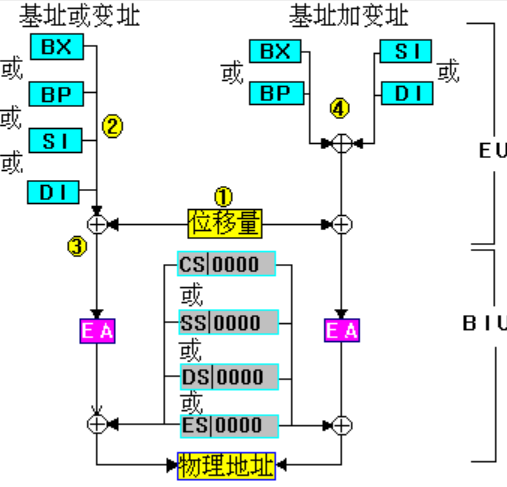
\includegraphics[scale=1]{part_指令系统/part_指令系统_pic/存储器物理地址计算图示.png}
    \caption{存储器物理地址计算图示}
\end{figure}
段寄存器可以是CS,SS,DS,ES;有效地址EA可以是
\begin{enumerate}
    \item 指令中直接指定的16位直接位移量,要加方括号
    \item BX/BP/SI/DI,{\color{red}{出现BP(不管是源处还是目的处)时默认使用SS提供段基址,但允许使用段超越前缀将SS修改为CS/DS/E,没有BP的,默认使用DS}}
    \item 位移量+基址/变址
    \item [BX/BP]+[SI/DI]+位移量,{\color{red}{画斜线的两者不能同时出现}}
\end{enumerate}
EA的24种表示法\ref{EA的24种表示方法}
\begin{figure}[H]
    \centering 
    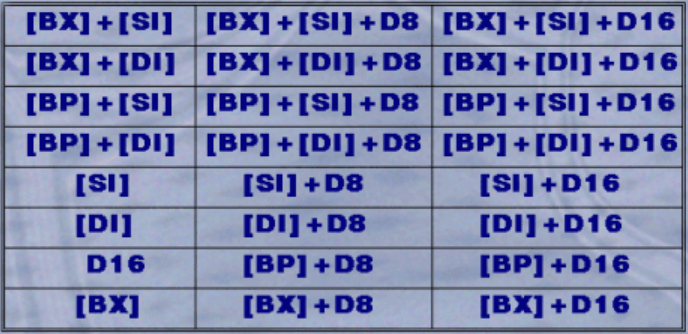
\includegraphics[scale=1]{part_指令系统/part_指令系统_pic/EA的24种表示方法.png}
    \caption{EA的24种表示方法}
    \label{EA的24种表示方法}
\end{figure}
\subsection{其他}
\subsubsection{隐含寻址}
指令中不明确指明操作数,但有隐含规定的 寻址方式。如:DAA对AL中的数进行十进制调整;CLI对中断标志清零
\subsubsection{一条指令包含几种寻址方式}
例如
\begin{lstlisting}
    MUL DL 
    ; AX<-AL*DL,源操作数为寄存器和隐含的寄存器AL
\end{lstlisting}
\subsubsection{IO端口寻址}
直接端口寻址:端口地址由指令直接给出,范围是00-FFH,若超出要先放到寄存器里。如
\begin{lstlisting}
    IN AL,40H
    OUT 83H,AL
\end{lstlisting}
间接端口寻址:端口地址由DX寄存器提供,其范围为0000-FFFFH
\begin{lstlisting}
    MOV DX,2F0H
    IN AL,DX ;;2F0H读入到AL
    MOV DX,300H
    OUT DX,AL ;;AL输出到300H
\end{lstlisting}
\subsubsection{转移类指令寻址}
详见控制转移指令
\section{数据传送}
\subsection{通用传送}
\subsubsection{MOV}
将操作数(字或字节)传送到目标操作数,源可为8位/16位通用寄存器(包括AX-DX,SI,DI,BP,SP),段寄存器(CS不能作为目的操作数),存储器或立即数。目的操作数不能为立即数,其他同源操作数。
四种数据来源的传送关系如图\ref{MOV指令的数据来源}
\begin{figure}[H]
    \centering 
    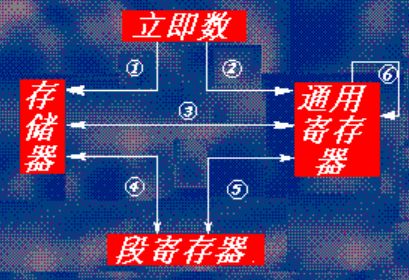
\includegraphics[scale=1]{part_指令系统/part_指令系统_pic/MOV指令的数据来源.png}
    \label{MOV指令的数据来源}
    \caption{MOV指令的数据来源}
\end{figure}
下面是一些示例
\begin{lstlisting}
    ; 立即数送存储器
    MOV [BX],0FFH
    ; 立即数送通用存储器
    MOV AL,30H
    MOV BL,'$'
    MOV AX,1250H
    MOV BX,OFFSET TABLE
    ; 存储器和通用寄存器相互传送
    MOV [BP],BX ; 带方框表示是段加偏移对应的存储器单元而不是BP本身的值受到改变
    MOV CL,5[BX]
    ; 存储器与段寄存器之间相互传送
    MOV [SI],DS
    ; 段寄存器和通用寄存器相互传送
    MOV ES,AX
    ; 通用寄存器之间相互传送
    MOV AX,DX
\end{lstlisting}
常见错误
\begin{lstlisting}
    ; 立即数不能作目的地
    MOV 60H,AL
    ; 存储器之间不能直接传送
    MOV [BX],[SI]
    ; CS不能作目的操作数
    MOV CS,AX
    ; 通用寄存器无IP寄存器
    MOV BX,IP
    ; 段寄存器之间不能直接传送
    MOV DS,ES 
    ; 数的长度不一致
    MOV CX,AL
\end{lstlisting}
\subsubsection{PUSH}
将源操作数入栈并使SP减二.{\color{red}低位先入栈}
\begin{lstlisting}
    PUSH AX ; 把AX入栈
\end{lstlisting}
\subsubsection{POP}
将当前SP指向的栈顶的一个字送到目的操作数中,并使SP+2.操作数可以是16位通用寄存器,DS/SS/ES或存储单元。{\color{red}堆栈操作总是以字为单位}
\begin{lstlisting}
    POP AX ; 先出栈的一个字节给到低位
\end{lstlisting}
\subsubsection{XCHG}
把字或字节的源操作数和目的操作数交换。可以发生在寄存之间或寄存器与存储器之间,但是段寄存器不能作操作数。
\begin{lstlisting}
    ; Right
    XCHG AX,BX
    XCHG [BI],CL 
    ; Wrong
    XCHG AX,0AF4H ;立即数不能交换
    XCHG SS,[SI] ; 段寄存器不参与交换
    XCHG [SI],[BX+1] ; 存储器之间不能直接交换
\end{lstlisting}
\subsubsection{XLAT}
将一个字节从一种代码转换成另一种代码。注意:
\begin{enumerate}
    \item 使用指令前必须先创建一个表格,将转换表的起始地址装入BX中
    \item AL存表头地址到所查找的某一项之间的位移量,根据位移量从表中查到转换后的代码值送入AL
    \item 表中最多存256字节
\end{enumerate}
典型的例子是用该指令将十进制数转换成七段显示管的代码
\begin{lstlisting}
    TABLE: DB 40H,79H,24H,30H,19H
           DB 12H,02H,78H,00H,18H ; 做表
           ... 
        LEA BX,TABLE ; 把表头地址给BX
        MOV AL,5 ; 把表内的偏移量给AL
        XLAT ; 此时AL中有‘5’的七段代码12H(表内从零开始数)
\end{lstlisting}
\subsection{输入输出}
\subsubsection{IN(OUT同理)}
把指定端口的内容读到AL(for byte)或AX(for word)中
\begin{lstlisting}
    ; 格式1:立即数指示端口
    IN AL,nn ;nn指代的8位端口的内容读到AL,nn=00-FFH
    IN AX,mm ;mm指代的16位端口读到AL,mm+1指代的16位端口读到AH.mm=00-FEH
    ; 格式2:用寄存器给端口号
    IN AL,DX ; DX=0000-FFFFH
    IN AX,DX ; DX=0000-FFFEH DX指代的16位端口读到AL,DX+1指代的16位端口读到AH
\end{lstlisting}
{\color{red}{当口地址大于FFH时,必须用格式2}}。典型示例:扬声器发声。
\subsection{地址目标}
这是一类专门用来传送地址码的指令
\subsubsection{LEA}
取源操作数地址的偏移量,传送到目的操作数所在的单元(load effective address)。{\color{red}源操作数必须是存储单元,目的操作数必须是除段寄存器以外的16位寄存器}
\begin{lstlisting}
    ; 注意区分LEA(取偏移地址)和MOV(取内容)
    ; 设SI=1000,DS=2000,(21000H)=1234,则
    LEA BX,[SI] ; BX=1000
    MOV BX,[SI] ; BX=1234
    ; 下面两段代码等效
    LEA BX,TABLE
    MOV BX,OFFSET TABLE
\end{lstlisting}
\subsubsection{LDS}
load DS:从源操作数指定的存储单元中取出4个字节的地址指针送进一对目的寄存器中(常用SI寄存器,但是不能是段寄存器)
load ES:与LDS基本相同但是后两个字节给到ES而非DS,目的操作数也常为DI而非SI
\begin{lstlisting}
    ; 设DS=0100,BX=0020,(01020H)=26A0H,(01022H)=B500H
    LDS SI,[BX] ; 低位两个字节给SI,SI=26A0,高位两字节给DS,DS=B500
    LES DI,[BX] ; DI=26A0,ES=B500
\end{lstlisting}
\subsection{标志传送}
\subsubsection{LAHF}
load AH flags:将SF,ZF,AF,PF,CF送到AH的7,6,4,2,0位,而5,3,1位为任意值。
\subsubsection{SAHF}
send AH flags:将AH的7,6,4,2,0位送到SF,ZF,AF,PF,CF,而高位flag(OF,DF,IF,TF)不受影响。
\subsubsection{PUSHF/POPF}
将整个标志寄存器的内容压栈/出栈,并使SP-2/+2(仍然是低位先入栈,高位先出栈)
\section{算数运算}
该类所有指令如图\ref{算数运算指令}
\begin{figure}[H]
    \centering 
    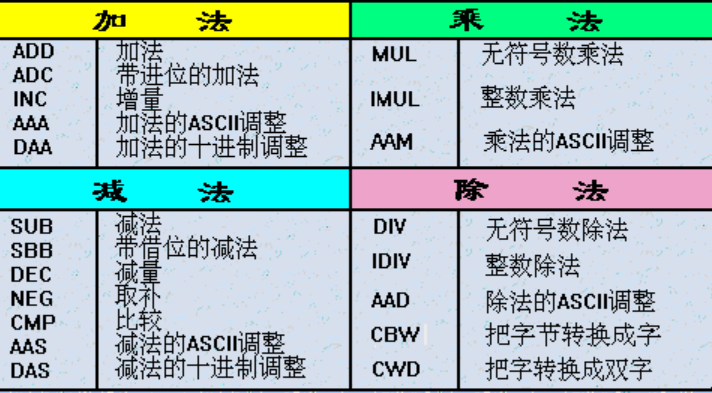
\includegraphics[scale=1]{part_指令系统/part_指令系统_pic/算数运算指令.png}
    \label{算数运算指令}
    \caption{算数运算指令}
\end{figure}
\subsection{加法}
\subsubsection{ADD}
目的数被赋值为“目的数+源”
\begin{lstlisting}
    ; RIGHT
    ADD AL,45H
    ADD BL,DL 
    ADD [BX],CL
    ; Wrong
    ADD 85H,AL ; 立即数不能被赋值
    ADD 5[BX],[BP] ; 两个存储器内容不能直接相加
    ADD BX,CL ; 字节和字不能相加
\end{lstlisting}
加法指令结束后将影响六个标志位,如何解释这些标志位(是无符号数相加还是有符号数相加决定是进位还是溢出)取决于程序员。
\subsubsection{ADC}
add carry:带进位的加法指令。目的=目的+源+CF
\subsubsection{INC}
increment:增量指令,对目的操作数加1.操作后影响AF,OF,PF,SF,ZF,但不影响CF
\begin{lstlisting}
    INC BL 
    INC BYTE PTR[BX] ; 对内存字节单元内容+1
    INC WORD PTR[BX] ; 对内存字单元内容+1
\end{lstlisting}
\subsubsection{AAA}
ascii-adjusted add:加法的ASCII调整指令。用ADD或ADC对两个非压缩十进制数或ASCII表示的十进制数作加法,且运算结果保留在AL中后,用AAA可以将运算结果调整为一位非压缩十进制数,仍然放在AL中。若AF=1,则表示高位有进位,进到AH中。

*非压缩十进数(BCD数):高四位全为零
例题图\ref{AAA指令例题}
\begin{figure}[H]
    \centering 
    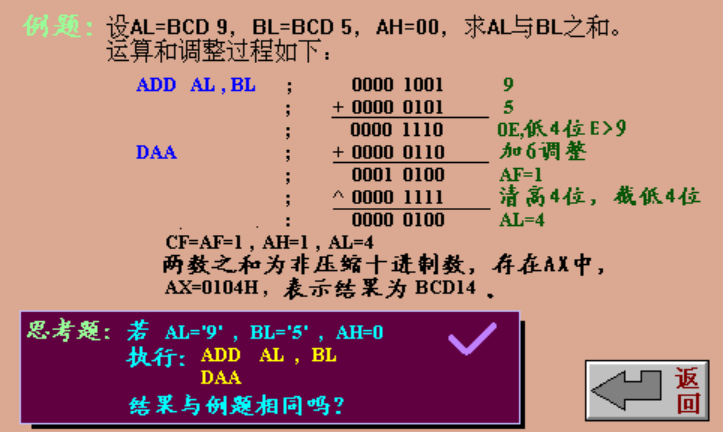
\includegraphics[scale=1]{part_指令系统/part_指令系统_pic/AAA指令例题.png}
    \label{AAA指令例题}
    \caption{AAA指令例题}
\end{figure}
\subsubsection{DAA}
decimal-adjusted add:加法的十进制调整指令。将两个压缩的BCD数相加的结果调整为正确的压缩BCD数,相加结果必须在AL中才能使用DAA。
例题图\ref{DAA指令例题}
\begin{figure}[H]
    \centering 
    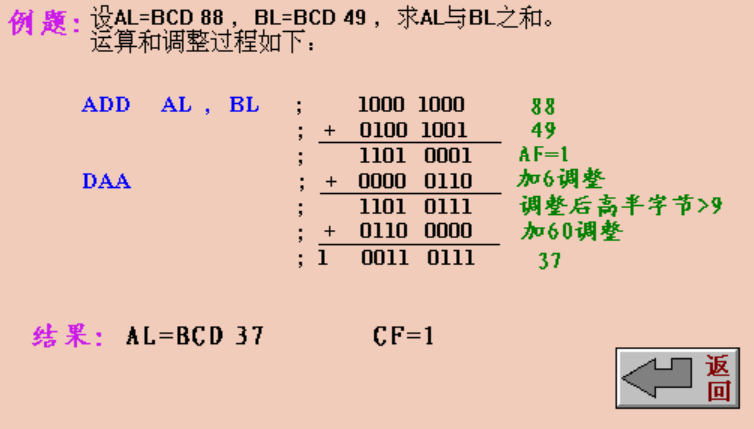
\includegraphics[scale=1]{part_指令系统/part_指令系统_pic/DAA指令例题.png}
    \label{DAA指令例题}
    \caption{DAA指令例题}
\end{figure}
\subsection{减法}
\subsubsection{SUB}
将目的操作数减去源操作数,结果送回目的操作数
\begin{lstlisting}
    SUB AL,BL ; 将AL-BL的值送到AL
\end{lstlisting}
\subsubsection{SBB}
带借位的减法:两个操作数相减后还要减去进位/借位标志CF的值,返回到目的操作数
\begin{lstlisting}
    SUB AL,CL ; 将AL-CL-CF的值送到AL
\end{lstlisting}
\subsubsection{DEC/NEG}
decrease:减量指令,对目的操作数减1,结果送回目的操作数。
\begin{lstlisting}
    DEC BX ; BX-1的值返回到BX
    DEC WORD PTR[BP] ; 堆栈段中位于[BP]偏移量处的字减1
\end{lstlisting}
negative:取反指令,即用0减去操作数再送回
\begin{lstlisting}
    MOV AL,00000101B ; AL=5
    NEG AL ;AL=11111011B (-5的补码)
\end{lstlisting}
\subsubsection{CMP}
compare:将目的数减去源操作数,结果不返回,但是反映在标志位上。这种指令用于希望在不破坏原数的情况下比较大小
\subsubsection{AAS/DAS}
ascii-adjusted sub:减法的ASCII调整。在减法指令后对两个非压缩的十进制数或ASCII码表示的十进制数相减后,在AL中得到的结果进行调整,使AL中得到正确的非压缩十进制数之差,若有借位,则CF置一。

低四位大于9/或AF=1时,用减6(而非+6)调整。

DAS类似,但是当当高4位大于9时,要减60H调整。
\subsection{乘法}
\subsubsection{MUL}
把源操作数和累加器中的数都当成无符号数。源操作数可以是字节或字
\begin{lstlisting}
    MUL DL ; DL*AL的结果放到AH(高)和AL(低)中
    MUL DX ; DX*AX的结果放到DX(高)和AX(低)中
\end{lstlisting}
\subsubsection{IMUL}
integer mul:整数乘法指令。把源和累加器中的数都当作有符号数相乘。若执行IMUL指令后,乘积的高半部分不是低半部分的符号扩展,则表示高位为有效位,是积的一部分,于是置CF=1,OF=1.若高半部分全是0或1,表明仅包含了符号位,CF=0,OF=0。
\subsubsection{AAM}
ascii-adjusted mul:乘法的ascii调整。对已经存放在AL中的两个非压缩的十进制数相乘的结果进行十进制数的调整,使得在AX中得到正确的非压缩十进制数的乘积。高位放在AH,低位放在AL。
\subsection{除法}
\subsubsection{DIV}
\begin{lstlisting}
    DIV BL ; AX/BL,商放在AL,余数放在AH
    DIV BX ; 若源操作数是字,则32位被除数放在DX(高)和AX中,相除后商放在AX,余数放在DX
\end{lstlisting}
如果被除数只有8位,则必须将其放在AL中,并把AH清零。如果被除数只有16位,则必须将其放在AX中,并把DX清零。{\color{red}{DIV执行后,所有标志无定义}}
\subsubsection{IDIV}
整数除法(带符号位除法):操作数、商和余数全是带符号数,并且规定余数的符号与被除数相同。所有标志位无定义。

{\color{red}{若被除数的高位绝对值大于除数的绝对值,也即商数超过了目标寄存器所能存放的数的范围,则计算机会出现除法错中断,商和余数不确定}}
\subsubsection{CBW}
把寄存器AL中的符号位扩充到AH的所有位,这是AH称为AL的符号扩充。即若AL的$D_7=0$,则AH的所有位都置零。反之都置一。
\subsubsection{CWD}
把AX的符号位扩充到DX中。
\subsubsection{AAD}
除法的ASCII调整:在做除法之前,把(AX中的)BCD码转化位二进制数。即执行AAD后,AL=AH*10+AL,AH=00H
\section{逻辑移位}
该类所有指令如图\ref{逻辑运算与移位指令}
\begin{figure}[H]
    \centering 
    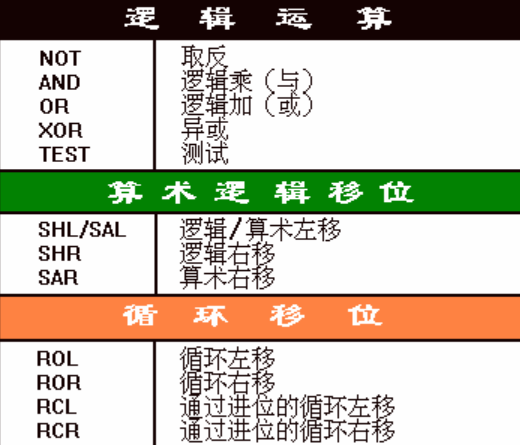
\includegraphics[scale=1]{part_指令系统/part_指令系统_pic/逻辑运算与移位指令.png}
    \label{逻辑运算与移位指令}
    \caption{逻辑运算与移位指令}
\end{figure}
\subsection{逻辑运算}
\subsubsection{NOT}
按位取反,返回到原位置
\subsubsection{AND,OR,XOR}
按位与/或/异或,结果返回到目的操作数
\subsubsection{TEST}
对两个操作数逻辑与,并修改标志位但不送回结果,操作后两个操作数都不变。往往后接转移指令。
\subsection{算数移位}
一般格式:“指令 目的,计数值”。计数次数=1时可以直接给出,否则要先把计数值送到CL
\subsubsection{SAL/SHL}
shift (arithmetic) left:将寄存器或存储器中的目的操作数各位左移,每移位一次,最低有效位LSB补零,最高有效位MSB进入CF。SHL与SAL一样。
\subsubsection{SHR}
shift right:将寄存器或存储器中的目的操作数各位右移,每移位一次,最低有效位LSB进入CF,最高有效位MSB补零。SHL与SAL一样。
\subsubsection{SAR}
与SHR类似。只是最高位不是补零而是保持不变。每移位一次相当于带符号数除以2.
\subsection{循环移位}
\subsubsection{ROL}
rotate left:循环左移。最高位不止给CF,还给到最低位
\subsubsection{ROR}
rotate right:循环右移。最低位不止给CF,还给到最高位
\subsubsection{RCL}
rotate carry left:通过进位位循环左移。把进位位放在最高位的左边一起参与左移。RCR也是是把进位位放在最高位的左边,一起参与右移。
\section{字符串}
字符串操作指令共有5条,每条指令有3种格式,指令后加B是字节操作,加W是字操作。

字符串指令隐含约定:
\begin{enumerate}
    \item 源串起始地址位DS:SI,允许用段超越前缀修改段地址DS
    \item 目的串起始地址为ES:DI,禁止使用段超越前缀修改ES
    \item 每次执行一次字符串指令,指针SI和DI自动修改
    \item DF标志位控制字符串处理方向。CLD使DF为0,为递增方向;STD使DF为1,递减。字节串每次SI,DI变1,字串每次变2
    \item 要处理的字符串长度放在CX寄存器中。可以在基本字符串指令前加重复前缀,加快串运算指令的执行速度。
\end{enumerate}
\subsection{传送}
\subsubsection{MOVS}
mov string
\begin{lstlisting}
    MOV CX,4 ;即要传送的字节数为4
    CLD ; 使DF=0,自增方向
    REP MOVSB ; 将DS:SI中的四个字节送到ES:DI中
\end{lstlisting}
\subsubsection{重复前缀}
\begin{enumerate}
    \item REP 常与MOVS或STOS连用
    \item REPE/REPZ 相等/结果为零则重复,常与CMPS连用,重复比较串数据知道两个字符不相等或CX=0
    \item REPNE/REPNZ 不相等/结果非零则重复。常与SCAS连用,重复查找某个数据知道ZF=1(找到了)或CX=0
\end{enumerate}
\subsection{比较}
\subsubsection{CMPS/CMPSB/CMPSW}
将源串内容减去目的串,并自动修改SI、DI,比较结果反映在FLAGS上,用来比较两个字符串是否相等。常用于密码验证
\begin{lstlisting}
    MOV CX,4
    CLD
    REPZ CMPS ; 将DS:SI指向的源串减去ES:DI指向的 目的串,若两串当此比较结果相同,ZF=1且CX不为零,则继续比较
\end{lstlisting}
\subsection{扫描}
\subsubsection{SCAS}
scan string:字符串扫描指令,从AL或AX寄存器的内容减去附加段中以DI为指针的目的元素,结果反映在标志位上,但是不改变操作数。被搜索的字(节)称为关键字
\begin{lstlisting}
    MOV DI,OFFSET STRING ;字串偏移地址
    MOV CX,COUNT ; 字符串长度即为最大重复次数
    MOV AL,'A' ; 关键字送入AL
    CLD
    REPNE SCASB 
    JZ FIND ; 搜索到,转出
    MOV DI,0 ; 没找到,DI=0
    FIND:
    MOV BX,DI ; BX=搜索次数
    HLT ; 停机
\end{lstlisting}
\subsection{装入}
\subsubsection{LODS}
load string:字符串装入指令。将DS:SI指向的源串送到AX(对字)或AL(对字节)中,并修改SI,加重复前缀无意义,因为累加器只能存储一个数据,重复操作后也只保留最后写入的数据。
\subsection{存储}
\subsubsection{STOS}
store string:数据串存储指令,与LODS相对。将累加器AL或AX中的一个字节或字传送到附加段中以DI为目标指针的目的串中,同时修改DI,以指向串中的下一个单元。与REP连用,常用于重复使用累加器中的一个常数,将串初始化(比如置为全0)
\begin{lstlisting}
    ; 设DI=2000H 
    MOV AX,0000H 
    CLD 
    STOSW ; 这一步执行完后,DI=2002H
    MOV AX,00FFH
    MOV CX,100H
    REP LODSW ???!!!; 这一步执行完后,DI=2202H,从ES:2002到ES:2201,全部装入00FFH
\end{lstlisting}
\section{控制转移}
该类所有指令如图\ref{控制转移指令}
\begin{figure}[H]
    \centering 
    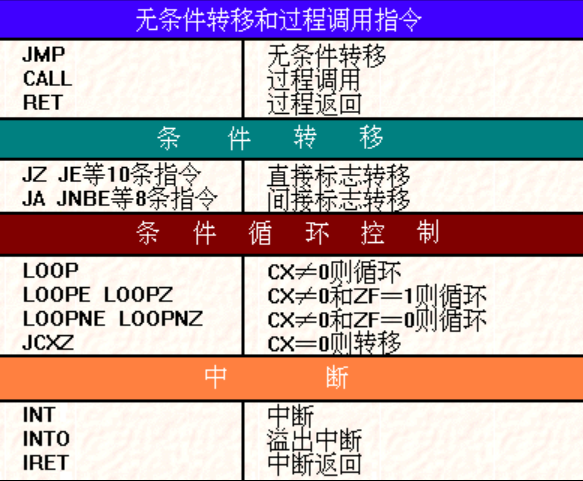
\includegraphics[scale=1]{part_指令系统/part_指令系统_pic/控制转移指令.png}
    \label{控制转移指令}
    \caption{控制转移指令}
\end{figure}
\subsection{无条件转移}
\begin{table}
    \centering
    \begin{tabular}{ccc}
        \hline 
        类型 & 方式 & 寻址目标  \\ \hline
        段内转移 & 直接 & 立即短转移(8位) \\ \hline
        段内转移 &直接& 直接近转移(16位)\\ \hline
        段内转移 & 间接 &寄存器(16位) \\ \hline
        段内转移 & 间接 &存储器(16位)\\ \hline
        段间转移 & 直接 & 立即转移(32位) \\ \hline
        段间转移 & 间接 & 存储器(32位)\\ \hline
    \end{tabular}
\end{table}
\subsubsection{段内直接转移指令}
\noindentbf{JMP SHORT PROGS}
段内短转移指令:指令执行后,跳转到标号为PROGS处执行。PROGS的偏移地址和JMP指令后下条地址之间的范围在-128-+127之间
\noindentbf{JMP (NEAR PTR) PROG}
PROG的偏移地址和JMP指令后下条地址之间的范围在-32768-+32767之间,若超出这个范围,汇编语言自动用向回转移的方法解决。该指令可以使程序转移到段内任何位置执行。
\subsubsection{段内间接转移指令}
有效地址可以是寄存器也可以是存储器单元
\begin{lstlisting}
    JMP BX ; 假设BX=4500H,则指令执行后将IP赋值为4500H
\end{lstlisting}
\subsubsection{段间直接转移指令}
\begin{lstlisting}
    JMP FAR PTR PROG ; 执行后,PROG所在的段内偏移量给IP,段地址给CS,即程序转到PROG处执行
\end{lstlisting}
\subsubsection{段间间接转移指令}
\begin{lstlisting}
    JMP DWORD PTR [SI+0125H]
\end{lstlisting}
当程序执行到上述指令时,从DS:SI+0125H这一数据段单元中取出两个字,低位给到IP,高位给CS,从而转到新的代码段执行。
\subsection{过程调用}
程序将某些独立的程序段模块化,称为过程或子程序。用CALL能调用这些过程。过程执行完后通过RET返回主程序,RET可以带参数。

子程序以PROC开头,以EDNP结束,RET位于ENDP之前
\subsubsection{段内直接调用}
\begin{lstlisting}
    MAIN PROC FAR 
    ... 
    CALL SUBPRO ;调用子程序,CALL指令的后一条指令的IP入栈,转入子程序执行。
    ... 
    RET 
    SUBPRO PROC NEAR ;子程序,NEAR说明是近过程
    ... 
    RET  ; 返址出栈,CALL指令的下一条指令执行
    SUBPRO ENDP 
    MAIN ENDP ; MAIN看作是DOS调用的一个子过程,其属性必须为FAR
\end{lstlisting}
\subsubsection{段间直接调用}
\begin{lstlisting}
    SEGM SEGMENT ;程序段A
    ... 
    CALL SUMPRO ; 段内调用子过程
    SUBPRO PROC FAR ; 进入远过程,并用FAR说明 
    ... 
    RET ; 远返回,从栈中弹出双字CS:IP 
    SUBPRO ENDP ; 返回CALL的下一条指令执行
    ... 
    SEGM ENDS 
    SEGB SEGMENT ; 程序段B
    ... 
    CALL SUBPRO ; 调用程序段A中的远过程,CALL的下一条指令的CS:IP入栈,转入SUBPRO执行
    ... 
    ENDS 
    SEGB ENDS 
\end{lstlisting}
与JMP的对比
\begin{enumerate}
    \item CALL无短调用指令
    \item JMP指令执行后不再返回原程序
    \item CALL指令的RET带参数n表示从栈中弹出返址后,再从栈中弹出n(0000-FFFFH)个字节的数据
\end{enumerate}
\subsection{条件转移}
根据上一条指令执行后CPU设置的状态标志做测试条件决定是否转移,满足条件才转移。所有的条件转移指令均为短转,目的地址都用标号表示
\subsubsection{直接标志转移指令}
\begin{table}[H]
    \centering 
    \begin{tabular}{ccc}
        \hline 
        指令助记符 & 测试条件 & 指令功能 \\ \hline
        JC   &      CF=1& 有进位 \\
        JNC    & CF=0 &无进位\\
        JZ/JE& ZF=1 &结果为0/相等\\
        JNZ/JNE &ZF=0 &不为零/不相等\\
        JS& SF=1 &符号为正\\
        JNS& SF=0 &符号为负\\
        JO &OF=1& 溢出\\
        JNO& OF=0 &无溢出\\
        JP/JPE& PF=1 &奇偶位为1/为偶\\
        JNP/JPO& PF=0 &奇偶位为0/为奇\\ \hline
    \end{tabular}
\end{table}
\begin{lstlisting}
    ADD AL,BL
    JC NEXT ;此处若CF=1,则转到NEXT处执行
    ... 
    NEXT:MOV AL,BL
\end{lstlisting}
\subsubsection{间接标志转移指令}
不是简单的通过标志状态位来决定是否跳转。而是经过一定的逻辑运算(更贴近数学逻辑)
\begin{table}[H]
    \centering 
    \begin{tabular}{ccc}
        \hline 
        类别 & 指令助记符 & 指令功能 \\ \hline
        无符号数比较 & JA/JNBE & 高于/不低于等于\\
        无符号数比较 & JAE/JNB&高于等于/不低于\\
        无符号数比较 & JB/JNAE&低于/不高于等于\\
        无符号数比较 & JBE/JNA&低于等于/不高于\\
        带符号数比较 & JG/JNLE&大于/不小于等于\\
        带符号数比较 & JGE/JNL&大于等于/不小于\\
        带符号数比较 & JL/JNGE&小于/不大于等于\\
        带符号数比较 & JLE/JNG&小于等于/不大于\\ \hline
    \end{tabular}
\end{table}
带符号数比较时,负数视为小于正数。
\subsection{条件循环控制}
增强型的条件转移指令,用于控制一个程序段的重复执行,重复次数在CX中
\subsubsection{LOOP}
后加短标号,循环标号指定程序CX次
\begin{lstlisting}
    MOV CX,8
    MOV BX,00 
    NEXT:MOV AL,[BX];加法程序 
    ADD AL,5
    MOV [BX],AL 
    INC BX 
    LOOP NEXT ;一共做8次加法
\end{lstlisting}
\subsubsection{LOOPE/LOOPZ}
相等或结果为零则循环指令
\subsubsection{LOOPNE/LOOPNZ}
不相等结果不为0则循环指令
\subsubsection{JCXZ}
若CX=0则跳转指令,主要用在循环程序开始处,为了使程序跳过循环,只要事先把CX清零即可
\subsection{中断指令}
\subsubsection{INT n}
软中断指令,将标志寄存器FLAGS内容入栈。断点(INT n的下条指令)基址:偏移地址入栈。从n*4开始的单元中取出中断服务程序入口地址的CS:IP转相应程序执行
\subsubsection{IRET}
中断返回指令,总是被安排在中断服务程序的出口处。功能是:
\begin{enumerate}
    \item 从栈中弹出断点送到CS和IP中
    \item 弹出FLAGS内容
    \item 按CS:IP的值返回断点,执行原来的程序
\end{enumerate}
\subsubsection{INTO}
溢出中断指令。当溢出标志OF=1,再执行INTO时,自动产生类型号为4的中断指令。即执行INT 4指令 

主要用于带符号数加减运算产生溢出错时的处理
\begin{lstlisting}
    ADD AL,BL 
    INTO ;如OF=1,则产生INT 4中断。此处若不安排INTO,溢出也不会产生中断,可能引发未知后果
\end{lstlisting}
\section{控制指令}
该类所有指令如图\ref{控制指令}
\begin{figure}[H]
    \centering 
    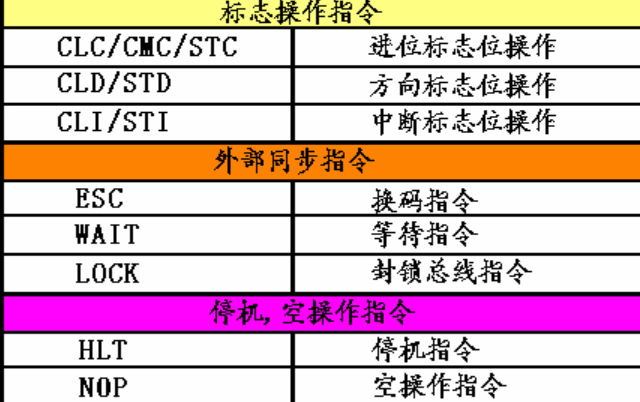
\includegraphics[scale=1]{part_指令系统/part_指令系统_pic/控制指令.png}
    \label{控制指令}
    \caption{控制指令}
\end{figure}
\subsection{标志操作指令}
这类指令可以直接对一些标志位进行操作。
\begin{table}[H]
    \centering 
    \begin{tabular}{cc}
        \hline 
        指令助记符 & 作用 \\ \hline 
        CLC &CF=0\\
        CMC &CF=$\overline{CF}$\\
        STC &CF=1\\
        CLD &DF=0(增量)\\
        STD &DF=1(减量)\\
        CLI &IF=0(不响应可屏蔽中断)\\
        STI &IF=1(响应可屏蔽中断)\\ \hline 
    \end{tabular}
\end{table}
\subsection{外部同步指令}
\subsubsection{ESC}
换码指令:协处理器8087和8086系统总线互联。一旦取出一条ESC指令,8087的BUSY引脚信号变高,通过它使8086的$\overline{TEST}$变高,协处理开始工作。完毕后向8086的$\overline{TEST}$发出低电平,执行后续指令。
\subsubsection{WAIT}
等待指令。通常跟在ESC之后。CPU执行ESC后,CPU处于等待状态,期间不断检测$\overline{TEST}$引脚,若为高,则重复执行WAIT。
\subsubsection{LOCK}
封锁总线指令。这是一种前缀,可加在任何指令的前端使8086的总线封锁信号有效。带有LOCK前缀的指令在执行过程中将禁止其他处理器使用总线
\begin{lstlisting}
    LOCK MOV AX,05H ;封锁总线指令
\end{lstlisting}
\subsection{停机和空操作}
\subsubsection{HLT}
停机指令。使CPU进入暂停状态,不进行任何操作。当下列情况之一发生时脱离暂停状态。常用HLT指令等待中断的出现
\begin{enumerate}
    \item 在RESET线上加复位信号
    \item NMI引脚上有中断请求信号
    \item 当IF=1,INTR引脚上出现中断请求信号时
\end{enumerate}
\subsubsection{NOP}
空操作或无操作指令。不完成任何操作。通常被插在其他指令之间,在循环等操作中增加延时。